\documentclass[11pt,a4paper]{article}
\usepackage[utf8]{inputenc}
\usepackage{amsmath,amssymb,amsthm}
\usepackage{hyperref}
\usepackage{booktabs}
\usepackage{listings}
\usepackage{xcolor}
\usepackage{tikz}
\usetikzlibrary{arrows.meta,positioning,shapes.geometric}
\usepackage[margin=2.5cm]{geometry}

\theoremstyle{definition}
\newtheorem{definition}{Definition}[section]
\newtheorem{theorem}{Theorem}[section]
\newtheorem{lemma}[theorem]{Lemma}
\newtheorem{corollary}[theorem]{Corollary}
\newtheorem{proposition}[theorem]{Proposition}
\newtheorem{remark}{Remark}[section]
\newtheorem{example}{Example}[section]

\definecolor{leanblue}{RGB}{0,0,180}
\definecolor{leankw}{RGB}{180,0,180}
\definecolor{leancomment}{RGB}{0,128,0}
\definecolor{leanstring}{RGB}{180,0,0}

\lstdefinelanguage{Lean}{
  morekeywords={def,theorem,lemma,where,by,intro,exact,apply,rw,simp,have,let,fun,match,with,if,then,else,structure,class,instance,extends,namespace,open,variable,axiom,sorry,Prop,Type,Set,Fin,Measure,List,Finset,ENNReal,ProbabilityMeasure,IsProbabilityMeasure},
  morestring=[b]",
  morecomment=[l]{--},
  morecomment=[s]{\{-}{-\}},
  sensitive=true
}
\lstset{
  language=Lean,
  basicstyle=\ttfamily\small,
  keywordstyle=\color{leankw}\bfseries,
  commentstyle=\color{leancomment}\itshape,
  stringstyle=\color{leanstring},
  columns=flexible,
  breaklines=true,
  frame=single,
  backgroundcolor=\color{gray!5}
}

\title{Directing Measures and Markov Mixtures:\\[0.3em]
\large Formalizing Diaconis--Freedman 1980 in Lean~4}

\author{Mettapedia Project}
\date{April 2026}

\begin{document}
\maketitle

\begin{abstract}
We present a complete Lean~4 formalization of the Markov de~Finetti theorem
(Diaconis--Freedman 1980): every Markov-exchangeable, recurrent prefix measure
on a finite alphabet is a mixture of time-homogeneous Markov chains. The
formalization comprises 26,665 lines of Lean code with zero unproved
assumptions (\texttt{sorry}), building on a 43,683-line formalization of the
classical (i.i.d.) de~Finetti theorem. Key innovations include a directing
measure uniqueness lemma that transfers de~Finetti structure across measure
restrictions, and a carrier transport bijection that establishes start-state
invariance via trajectory segment swapping. The proof architecture decomposes
into successor-matrix partial exchangeability, per-row de~Finetti factorization,
and cross-row coherence induction. This formalization provides a verified
foundation for structured universal mixtures in the style of Solomonoff
induction, where Markov models replace i.i.d.\ hypotheses for tractable
sequential prediction.
\end{abstract}

\tableofcontents

\section{Introduction}

Solomonoff induction (1964) provides a universal Bayesian mixture over all
computable hypotheses. In practice, one restricts to structured hypothesis
classes---i.i.d.\ models, finite-state Markov models, hidden Markov
models---for tractability and interpretability. The conceptual bridge is:

\begin{quote}
\emph{Exchangeability (or partial exchangeability) assumptions identify when
a rich family of distributions can be represented as a mixture over a simpler
parametric family.}
\end{quote}

For i.i.d.\ sequences, de~Finetti's theorem (1931/1937) gives exchangeability
$\Rightarrow$ mixture of i.i.d.\ laws. For Markov sequences, Diaconis and
Freedman (1980) show a corresponding representation for \emph{Markov-exchangeability},
with an additional \emph{recurrence} hypothesis.

\subsection{The Theorem}

Let $A = \{0, 1, \ldots, k-1\}$ be a finite alphabet. A \emph{prefix measure}
$\mu$ assigns a nonnegative extended real to each finite word over $A$, satisfying
$\mu(\varepsilon) = 1$ and $\mu(xs) = \sum_{a \in A} \mu(xs \cdot [a])$. We say
$\mu$ is \emph{Markov-exchangeable} if $\mu(xs) = \mu(ys)$ whenever $xs$ and $ys$
have the same \emph{Markov evidence}: the starting state and transition-count matrix.

\begin{theorem}[Diaconis--Freedman 1980]\label{thm:df80}
Let $\mu$ be a Markov-exchangeable prefix measure on a finite alphabet $A$.
If $\mu$ satisfies a recurrence condition (the trajectory returns to its
starting state infinitely often, almost surely under any extension), then
there exists a probability measure $\pi$ on the space of Markov parameters
$\Theta_k = \Delta_k \times \Delta_k^k$ such that for all finite words $xs$:
\[
\mu(xs) = \int_{\Theta_k} \mathrm{wordProb}_\theta(xs) \, d\pi(\theta)
\]
where $\mathrm{wordProb}_\theta(x_0, x_1, \ldots, x_n) = \pi_0(x_0) \cdot \prod_{t=0}^{n-1} P(x_t, x_{t+1})$
is the Markov chain probability.
\end{theorem}

\subsection{Why Formalize?}

The Markov de~Finetti theorem is foundational for:
\begin{itemize}
\item \textbf{Bayesian sequential prediction}: Dirichlet-multinomial conjugacy
  for Markov chains, with dominance-style guarantees.
\item \textbf{PLN evidence aggregation}: The ``evidence is what you carry''
  design---under exchangeability, binary counts $(n^+, n^-)$ are sufficient
  statistics.
\item \textbf{Structured universal mixtures}: Solomonoff-like prediction
  instantiated over finite-state hypotheses with hyperpriors retaining
  universality guarantees.
\end{itemize}

The proof involves subtle measure-theoretic arguments: conditional independence
across row processes, almost-everywhere uniqueness of directing measures, and
carrier bijections preserving transition counts. Formalization provides
certainty that the intricate decomposition is correct.

\subsection{Contribution}

We present:
\begin{enumerate}
\item A complete formalization of Theorem~\ref{thm:df80} in Lean~4 with Mathlib:
  \textbf{26,665 lines}, \textbf{0 sorry}, \textbf{33 files}.
\item Reuse of a 43,683-line formalization of the classical de~Finetti theorem
  (three independent proofs: martingale, $L^2$, ergodic).
\item Key innovations:
  \begin{itemize}
  \item \emph{Directing measure uniqueness}: If $\nu \leq C \cdot \mu$ for
    exchangeable measures, their directing measures agree $\nu$-a.e.
  \item \emph{Carrier transport}: Trajectory segment swapping provides
    evidence-preserving bijections between visit-time fibers.
  \end{itemize}
\item A structural audit methodology that identified and closed three
  previously overlooked gaps in the proof architecture.
\end{enumerate}

\section{Mathematical Background}

\subsection{Prefix Measures}

A \emph{prefix measure} on $\mathrm{Fin}(k)$ is a function
$\mu : \mathrm{List}(\mathrm{Fin}(k)) \to [0, \infty]$ satisfying:
\begin{itemize}
\item $\mu([]) = 1$ (normalization)
\item $\mu(xs) = \sum_{a \in \mathrm{Fin}(k)} \mu(xs \cdot [a])$ (consistency)
\end{itemize}

In Lean:
\begin{lstlisting}
-- FiniteAlphabet.PrefixMeasure (Fin k)
-- A function List (Fin k) -> ENNReal satisfying consistency
\end{lstlisting}

\subsection{Transition Counts and Markov Evidence}

For a trajectory $xs : \mathrm{Fin}(n+1) \to \mathrm{Fin}(k)$, the
\emph{Markov evidence} consists of:
\begin{itemize}
\item The starting state $x_0$
\item The transition-count matrix $N(i,j) = \#\{t < n : x_t = i \land x_{t+1} = j\}$
\end{itemize}

\begin{lstlisting}
structure MarkovEvidence (k : Nat) where
  start : Fin k
  trans : Fin k -> Fin k -> Nat

def evidenceOf (xs : Fin (n + 1) -> Fin k) : MarkovEvidence k :=
  { start := xs 0,
    trans := fun a b => transCount xs a b }
\end{lstlisting}

\subsection{Markov Exchangeability}

\begin{definition}
A prefix measure $\mu$ is \emph{Markov-exchangeable} if for all $xs, ys$ of
the same length with $\mathrm{evidenceOf}(xs) = \mathrm{evidenceOf}(ys)$:
$\mu(xs) = \mu(ys)$.
\end{definition}

\begin{lstlisting}
def MarkovExchangeablePrefixMeasure
    (mu : PrefixMeasure (Fin k)) : Prop :=
  forall (n : Nat) (xs1 xs2 : Fin (n + 1) -> Fin k),
    evidenceOf xs1 = evidenceOf xs2 ->
      mu (List.ofFn xs1) = mu (List.ofFn xs2)
\end{lstlisting}

\subsection{The Markov Parameter Space}

A Markov model on $\mathrm{Fin}(k)$ is parameterized by:
\begin{itemize}
\item An initial distribution $\pi_0 \in \Delta_k$
\item $k$ row-stochastic transition distributions $P(i, \cdot) \in \Delta_k$
\end{itemize}

The parameter space $\Theta_k = \Delta_k \times \Delta_k^k$ is a finite product
of simplices, hence compact. The word probability function
$\theta \mapsto \mathrm{wordProb}_\theta(xs)$ is continuous on $\Theta_k$.

\subsection{Recurrence}

Markov exchangeability alone does \emph{not} imply a mixture representation.
A counterexample: the deterministic chain $0 \to 1 \to 1 \to 1 \to \cdots$
is Markov-exchangeable (trivially---equivalence classes are singletons) but
not a mixture of recurrent Markov chains.

\begin{definition}
A prefix measure $\mu$ is \emph{recurrent} if it admits an extension $P$ to
infinite sequences where the trajectory returns to its starting state
infinitely often, $P$-almost surely.
\end{definition}

\begin{lstlisting}
def recurrentEvent : Set (Nat -> Fin k) :=
  { omega | forall N, exists n >= N, omega n = omega 0 }

def MarkovRecurrentPrefixMeasure (mu : PrefixMeasure (Fin k)) : Prop :=
  exists (P : Measure (Nat -> Fin k)),
    IsProbabilityMeasure P /\
    (forall xs, mu xs = P (cylinder xs)) /\
    P recurrentEvent = 1
\end{lstlisting}

\section{The Formal Statement}

\subsection{Row-Kernel Crux Data}

The internal representation theorem requires \emph{row-kernel crux data}:
a family of row kernels with measurability, start-restriction, and coherence
properties.

\begin{lstlisting}
def RowKernelCruxData
    (P : Measure (Nat -> Fin k))
    (rowKernel : Fin k -> (Nat -> Fin k)
                 -> ProbabilityMeasure (Fin k)) : Prop :=
  -- (1) Singleton-eval AE-measurability
  (forall i b, AEMeasurable
    (fun r => (rowKernel i r) {b})
    (rowProcessLaw P i)) /\
  -- (2) Start-restricted invariance
  StartRestrictedRowKernelData P rowKernel /\
  -- (3) Product-kernel AE-measurability
  (forall i, AEMeasurable
    (fun r => Measure.pi (fun _ => rowKernel i r))
    (rowProcessLaw P i)) /\
  -- (4) Cross-row coherence step
  CrossRowCoherenceStep P rowKernel
\end{lstlisting}

\subsection{The Internal Representation Theorem}

\begin{theorem}[Internal Representation, \texttt{proved}]
\label{thm:internal}
Given an extension $P$ of a prefix measure $\mu$ with row-kernel crux data,
there exists a probability measure $\pi$ on $\mathrm{MarkovParam}(k)$ such that
$\mu(xs) = \int \mathrm{wordProb}_\theta(xs) \, d\pi(\theta)$.
\end{theorem}

\begin{lstlisting}
theorem fortiniSuccessorMatrixInvarianceTheoremInternal_proved :
    FortiniSuccessorMatrixInvarianceTheoremInternal k := by
  intro mu hP hExt rowKernel hcrux
  -- Construct pi as pushforward of P through
  -- omega |-> rowKernelToMarkovParam(omega)
  ...
\end{lstlisting}

\subsection{The Crown Theorem}

The full theorem derives the row-kernel crux data from Markov exchangeability
and recurrence alone.

\begin{lstlisting}
abbrev FortiniCanonicalRepresentationTheorem (k : Nat) : Prop :=
  forall mu : PrefixMeasure (Fin k),
    MarkovExchangeablePrefixMeasure mu ->
    MarkovRecurrentPrefixMeasure mu ->
      exists (pi : Measure (MarkovParam k)),
        IsProbabilityMeasure pi /\
        forall xs, mu xs = integral theta, wordProb theta xs dpi
\end{lstlisting}

\section{Proof Architecture}

The proof decomposes into two layers:

\begin{center}
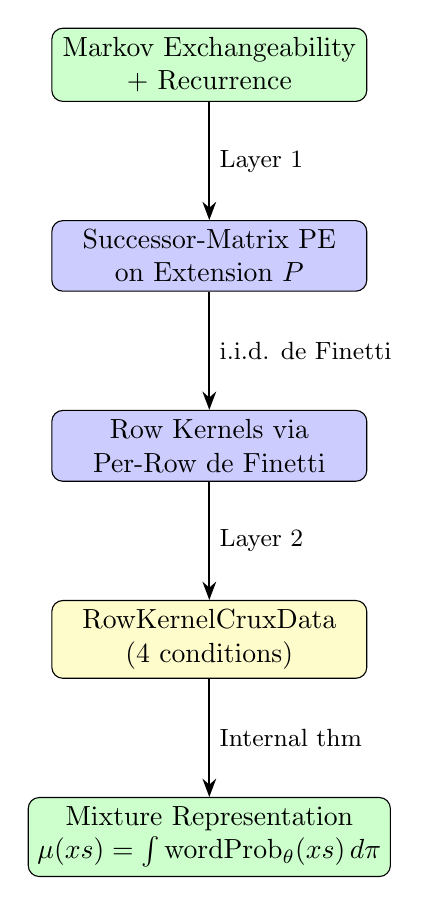
\begin{tikzpicture}[
  node distance=1.5cm,
  box/.style={rectangle, draw, rounded corners, minimum width=4cm, minimum height=0.8cm, align=center},
  arrow/.style={-{Stealth}, thick}
]
\node[box, fill=green!20] (me) {Markov Exchangeability\\+ Recurrence};
\node[box, fill=blue!20, below=of me] (pe) {Successor-Matrix PE\\on Extension $P$};
\node[box, fill=blue!20, below=of pe] (rk) {Row Kernels via\\Per-Row de Finetti};
\node[box, fill=yellow!20, below=of rk] (crux) {RowKernelCruxData\\(4 conditions)};
\node[box, fill=green!20, below=of crux] (mix) {Mixture Representation\\$\mu(xs) = \int \mathrm{wordProb}_\theta(xs) \, d\pi$};

\draw[arrow] (me) -- (pe) node[midway,right] {\small Layer 1};
\draw[arrow] (pe) -- (rk) node[midway,right] {\small i.i.d. de Finetti};
\draw[arrow] (rk) -- (crux) node[midway,right] {\small Layer 2};
\draw[arrow] (crux) -- (mix) node[midway,right] {\small Internal thm};
\end{tikzpicture}
\end{center}

\subsection{Layer 1: Successor-Matrix Partial Exchangeability}

A measure $P$ on $\mathbb{N} \to \mathrm{Fin}(k)$ is \emph{successor-matrix
partially exchangeable} if for every finite selection of anchor states and
visit indices, within-row permutations leave the joint law invariant.

\begin{lstlisting}
def SuccessorMatrixPartialExchangeable
    (P : Measure (Nat -> Fin k)) : Prop :=
  forall (m : Nat) (anchor : Fin m -> Fin k)
         (idx : Fin m -> Nat) (sigma : Fin k -> Equiv.Perm Nat),
    Measure.map
      (fun omega => fun j => rowSuccessorVisitProcess (anchor j) omega
                               ((sigma (anchor j)) (idx j))) P
    =
    Measure.map
      (fun omega => fun j => rowSuccessorVisitProcess (anchor j) omega
                               (idx j)) P
\end{lstlisting}

This is derived from Markov exchangeability via the carrier transport argument.

\subsection{Layer 2: Row-Kernel Construction}

From successor-matrix PE, each row's law $\mathrm{rowProcessLaw}(P, i)$ is
exchangeable in the classical sense. We apply the i.i.d.\ de~Finetti theorem
to extract the \emph{directing measure}:

\begin{lstlisting}
noncomputable def directingRowKernel
    (P : Measure (Nat -> Fin k)) (i : Fin k)
    (r : Nat -> Fin k) : ProbabilityMeasure (Fin k) :=
  directingMeasure (mu := rowProcessLaw P i)
    (fun n (r : Nat -> Fin k) => r n) measurability_proof r
\end{lstlisting}

\subsection{The Directing Measure Uniqueness Lemma}

A key innovation: if $\nu \leq C \cdot \mu$ for exchangeable probability
measures, then their directing measures agree $\nu$-almost everywhere.

\begin{lemma}[\texttt{directingMeasure\_singleton\_ae\_eq\_of\_smul\_le}]
\label{lem:unique}
Let $\mu, \nu$ be probability measures with $X : \mathbb{N} \to \Omega \to \alpha$
exchangeable under both. If $\nu \leq C \cdot \mu$ for some $C < \infty$, then
for all $b \in \alpha$:
\[
\mathrm{directingMeasure}_\mu(\omega)\{b\} =_{\nu\text{-a.e.}}
\mathrm{directingMeasure}_\nu(\omega)\{b\}
\]
\end{lemma}

This is crucial for showing that the directing kernel computed from the full
measure $P$ serves correctly for restrictions $P|_{\{\omega_0 = a\}}$.

\subsection{Start-Restricted Factorization}

The start-restricted invariance condition requires:
\[
\mathrm{rowProcessLaw}(P|_{\omega_0 = a}, i) \text{ factors through }
\mathrm{directingRowKernel}(P, i)
\]

The proof:
\begin{enumerate}
\item If $P(\omega_0 = a) = 0$: both sides are zero measures.
\item If $P(\omega_0 = a) = c > 0$: normalize $\rho_{a,\text{norm}} = c^{-1} \cdot \mathrm{rowProcessLaw}(P|_{\omega_0=a}, i)$.
  This is a probability measure, and exchangeable (inherited).
\item Apply the i.i.d.\ de~Finetti theorem to $\rho_{a,\text{norm}}$.
\item Apply Lemma~\ref{lem:unique}: $\rho_{a,\text{norm}} \leq c^{-1} \cdot \mathrm{rowProcessLaw}(P, i)$,
  so directing measures agree.
\item Scale back: the factorization identity holds for the unnormalized measure.
\end{enumerate}

\begin{lstlisting}
theorem startRestrictedRowKernelData_directingRowKernel
    (mu : PrefixMeasure (Fin k))
    (hmu : MarkovExchangeablePrefixMeasure mu)
    (P : Measure (Nat -> Fin k)) [IsProbabilityMeasure P]
    (hExt : forall xs, mu xs = P (cylinder xs))
    (hStrRec : StrongRecurrence P)
    (hExch : forall i, Exchangeable (rowProcessLaw P i)
               (fun n r => r n)) :
    StartRestrictedRowKernelData P (directingRowKernel P)
\end{lstlisting}

\subsection{Carrier Transport}

The start-restricted permutation invariance is derived from Markov
exchangeability via finite combinatorics:

\begin{enumerate}
\item Fix state $i$, target $b \neq i$, and visit indices $n, n+1$.
\item The \emph{carrier} is the set of length-$N$ prefixes consistent with
  a given visit-time event.
\item Construct a bijection between carriers by \emph{segment swapping}:
  transpose the excursion between the $n$-th and $(n+1)$-th visits with
  the excursion between the $(n+1)$-th and $(n+2)$-th visits.
\item This bijection preserves Markov evidence (start state + transition counts).
\item By Markov exchangeability, the two carriers have equal $\mu$-measure.
\item Taking $N \to \infty$ gives the start-restricted invariance.
\end{enumerate}

\begin{lstlisting}
theorem carrierTransportEquivAdjacent {N : Nat}
    (i : Fin k) (b : Fin k) (hbi : b != i) (n : Nat)
    (hSuff : sufficiency_hypotheses) :
    exists e : carrier(i, {n}, ..., N) <-> carrier(i, {n+1}, ..., N),
      forall xs, evidenceOf xs.1 = evidenceOf (e xs).1
\end{lstlisting}

\section{Key Lemmas}

\subsection{Directing Measure Uniqueness}

\begin{lstlisting}
theorem directingMeasure_singleton_ae_eq_of_smul_le
    [Fintype alpha] [MeasurableSingletonClass alpha]
    (X : Nat -> Omega -> alpha) (hX_meas : forall n, Measurable (X n))
    {mu nu : Measure Omega} [IsProbabilityMeasure mu]
                            [IsProbabilityMeasure nu]
    (hX_exch_mu : Exchangeable mu X)
    (hX_exch_nu : Exchangeable nu X)
    {C : ENNReal} (hC : C != top) (hle : nu <= C * mu)
    (b : alpha) :
    (fun omega => (directingMeasure (mu := mu) X hX_meas omega {b}).toReal)
    =ae[nu]
    (fun omega => (directingMeasure (mu := nu) X hX_meas omega {b}).toReal)
\end{lstlisting}

\textbf{Proof idea}: The directing measure is the a.e.\ limit of empirical
frequencies. Under $\nu \leq C \cdot \mu$, any $\nu$-a.e.\ property holds
$\mu$-a.e.\ on the support of $\nu$. The empirical frequency limits agree
on this common support.

\subsection{Start-Restricted Row-Kernel Data}

This is the theorem proved in the final session:

\begin{lstlisting}
theorem startRestrictedRowKernelData_directingRowKernel
    (mu : PrefixMeasure (Fin k))
    (hmu : MarkovExchangeablePrefixMeasure mu)
    (P : Measure (Nat -> Fin k)) [IsProbabilityMeasure P]
    (hExt : forall xs, mu xs = P (cylinder xs))
    (hStrRec : StrongRecurrence P)
    (hExch : forall i, Exchangeable (rowProcessLaw P i)
               (fun n r => r n)) :
    StartRestrictedRowKernelData P (directingRowKernel P) := by
  intro i a m sel hsel
  by_cases hc : P {omega | omega 0 = a} = 0
  -- Zero case: both sides are zero
  case pos => ...
  -- Positive case: normalize, apply de Finetti, use uniqueness
  case neg =>
    set c := P {omega | omega 0 = a}
    set rho_a := rowProcessLaw (P.restrict {...}) i
    set rho_a_norm := c^(-1) * rho_a
    -- rho_a_norm is a probability measure
    -- rho_a_norm is exchangeable
    -- Apply de Finetti to rho_a_norm
    -- Apply directing measure uniqueness
    -- Scale back to rho_a
    ...
\end{lstlisting}

\subsection{Carrier Transport Bijection}

\begin{lstlisting}
theorem carrierTransportEquivAdjacent {N : Nat}
    (i : Fin k) (b : Fin k) (hbi : b != i) (n : Nat)
    (hSuff : ...) :
    exists e : carrier(i, {n}, N) <-> carrier(i, {n+1}, N),
      forall xs, evidenceOf xs.1 = evidenceOf (e xs).1 := by
  -- Construct segmentSwap
  -- Prove self-inverse
  -- Prove evidence preservation
  -- Prove carrier membership preservation
  ...
\end{lstlisting}

\section{File Inventory}

All files are in \texttt{Mettapedia/Logic/} within the Mettapedia Lean project.

\begin{table}[h]
\centering
\begin{tabular}{llr}
\toprule
\textbf{Layer} & \textbf{File} & \textbf{Lines} \\
\midrule
Fiber bridge & MarkovDeFinettiFiberEventBridge.lean & 9,324 \\
Crux pipeline & MarkovDeFinettiFortiniBridgeCrux.lean & 2,853 \\
PE bridge & MarkovDeFinettiPEBridge.lean & 2,250 \\
Bridge core & MarkovDeFinettiFortiniBridgeCore.lean & 2,130 \\
Carrier transport & MarkovDeFinettiCarrierTransport.lean & 1,374 \\
Counterexample & MarkovDeFinettiFortiniCrossAnchorCounterexample.lean & 1,010 \\
Kernel uniqueness & MarkovDeFinettiKernelUniqueness.lean & 922 \\
Euler trails & MarkovDeFinettiHard*.lean (6 files) & 1,948 \\
Evidence basis & MarkovDeFinettiEvidenceBasis.lean & 305 \\
Moment problem & MarkovDeFinettiMomentProblem.lean & 287 \\
Higher-order Markov & MarkovDeFinettiHigherOrder.lean & 1,219 \\
Hidden Markov models & FiniteHiddenMarkovModel.lean & 668 \\
Higher-order Giry bridge & DeFinettiHigherOrderGiryBridge.lean & 175 \\
HMM de Finetti bridge & FiniteHiddenMarkovDeFinettiBridge.lean & 339 \\
Higher-order WM bridge & WMHigherOrderMarkov.lean & 365 \\
Controlled HMM/POMDP bridge & ControlledFiniteHiddenMarkovModel.lean, ControlledFiniteHiddenMarkovObservedInference.lean, ControlledFiniteHiddenMarkovBridge.lean & 827 \\
Controlled Solomonoff bridge & ControlledPrefixMeasure.lean, ControlledSolomonoffBridge.lean, ControlledFiniteHiddenMarkovUniversalPredictionBridge.lean & 446 \\
Other & (11 files) & 1,496 \\
\midrule
\textbf{Total} & \textbf{36 files} & \textbf{27,938} \\
\bottomrule
\end{tabular}
\caption{Markov de Finetti formalization file inventory}
\end{table}

\subsection{External Dependencies}

The formalization builds on the classical de~Finetti theorem, formalized in
\texttt{Mettapedia/external/exchangeability/} (43,683 lines, 0 sorry). This
provides three independent proofs:

\begin{enumerate}
\item \textbf{Via reverse martingale convergence} (default, follows Kallenberg 2005)
\item \textbf{Via $L^2$ bounds} (lightest dependencies, elementary)
\item \textbf{Via mean ergodic theorem} (connects to dynamical systems)
\end{enumerate}

\section{The Classical de Finetti Context}

The i.i.d.\ de~Finetti theorem states:
\[
\text{Contractable} \iff \text{Exchangeable} \iff \text{Conditionally i.i.d.}
\]
for infinite sequences on standard Borel spaces.

The Markov version replaces ``i.i.d.'' with ``time-homogeneous Markov chain''
and ``exchangeable'' with ``Markov-exchangeable.'' The additional recurrence
hypothesis is necessary to exclude deterministic transient behavior.

\subsection{Row-Process Decomposition}

The key bridge from Markov to i.i.d.\ is the \emph{row-process}:

\begin{definition}
For anchor state $i$ and trajectory $\omega$, the \emph{row-successor process}
$\mathrm{rsp}_i(\omega) : \mathbb{N} \to \mathrm{Fin}(k)$ records the state
visited \emph{after} the $n$-th visit to $i$:
\[
\mathrm{rsp}_i(\omega, n) = \omega(t_{n,i}(\omega) + 1)
\]
where $t_{n,i}(\omega)$ is the time of the $n$-th visit to state $i$.
\end{definition}

Under successor-matrix PE, each row process
$\mathrm{rowProcessLaw}(P, i)$ is exchangeable in the classical sense.
Applying the i.i.d.\ de~Finetti theorem row-by-row extracts the directing
measures that become the row kernels.

\section{Toward Solomonoff: Structured Universal Mixtures}

\subsection{The Solomonoff Connection}

Solomonoff's universal prior assigns:
\[
M(x_{1:n}) = \sum_{p : \text{program}} 2^{-|p|} \cdot \mathbf{1}[U(p) \text{ outputs } x_{1:n}]
\]
This is a mixture over all computable hypotheses.

The Markov de~Finetti theorem justifies a \emph{structured} version:
\[
\mu(x_{1:n}) = \int_{\Theta_k} \mathrm{wordProb}_\theta(x_{1:n}) \, d\pi(\theta)
\]
where $\pi$ is a (possibly universal) prior on Markov parameters. Under
Markov exchangeability, this representation exists and is unique.

\subsection{Dominance Guarantees}

A universal hyperprior over Dirichlet priors (one per transition row) gives:
\begin{itemize}
\item Conjugate Bayesian updates via count aggregation
\item Dominance over all finitely parameterized Markov predictors
\item Computable inference via the Dirichlet-multinomial formula
\end{itemize}

This is formalized in \texttt{MarkovDirichletHyperpriorMixture.lean}.

\subsection{PLN Evidence Aggregation}

The count-sufficiency result---under exchangeability, $\mu(xs)$ depends only
on $\mathrm{evidenceOf}(xs)$---justifies PLN's ``evidence is what you carry''
design. Binary evidence $(n^+, n^-)$ is sufficient for exchangeable binary
sequences; transition counts $N(i,j)$ are sufficient for Markov-exchangeable
sequences.

\subsubsection{The PLN-Markov Bridge}

PLN (Probabilistic Logic Networks) represents uncertain knowledge via
truth-value pairs $(s, c)$ where $s$ is strength and $c$ is confidence.
The Markov de~Finetti theorem provides the measure-theoretic foundation
for PLN's evidence-based reasoning in sequential domains:

\begin{enumerate}
\item \textbf{Evidence sufficiency}: Under Markov exchangeability,
  the transition-count matrix $N(i,j)$ is a sufficient statistic.
  PLN's evidence aggregation rules (count addition, forgetting via
  set difference) are justified by this sufficiency.
\item \textbf{Dirichlet conjugacy}: The posterior over Markov parameters
  given transition counts follows a product-Dirichlet distribution.
  This is formalized in \texttt{EvidenceDirichlet.lean} and underlies
  PLN's Bayesian update rules.
\item \textbf{Predictive inference}: Given evidence $N$, the predictive
  distribution for the next transition $i \to j$ is
  $\frac{N(i,j) + \alpha}{\sum_k N(i,k) + k\alpha}$ (Laplace smoothing).
  This is the ``strength'' in PLN terms, with confidence derived from
  total count.
\end{enumerate}

The formalization connects these three layers: the representation theorem
(\S4) justifies evidence sufficiency, the Dirichlet infrastructure
(\texttt{MarkovDirichletPredictor.lean}) provides conjugate updates,
and the hyperprior mixture (\texttt{MarkovDirichletHyperpriorMixture.lean})
gives Solomonoff-style dominance guarantees.

\medskip

\noindent\textbf{Current theorem surface (2026-04):} the post-Markov bridge is
now exposed at three abstraction levels:
\begin{enumerate}
\item \textbf{General $k$-ary}: \texttt{markovExchangeable\_domain\_characterization}
  shows the sufficient statistic is $(\mathrm{counts}, \mathrm{last})$
  (\texttt{MarkovExchangeabilityBridge.lean}).
\item \textbf{Binary presentations}: Both \texttt{Fin 2} and explicit Boolean
  $(ff,ft,tf,tt,\mathrm{lastBit})$ with witness-based Solomonoff wrappers and
  direct Markov $\nu$PLN master-chain theorems.
\item \textbf{Class-recurrence}: \texttt{MarkovBinaryPLNDomainConditionsInClass}
  packages binary domain conditions under class recurrence, with
  \texttt{Fin 2} and \texttt{Bool} row-law factorization theorems
  (\texttt{SolomonoffExchangeable.lean:590--802}). The downstream theorems
  are scoped to $i \in C$, which is the honest mathematical scope.
\end{enumerate}
The class-recurrence layer enables PLN-style reasoning in settings where only
partial recurrence is known, with explicit tracking of which transition rows
support the factorization.

\subsubsection{The Markov Xi Transition Surface}

The formalization exposes a direct transition atom surface via
\texttt{MarkovTransitionXi.lean} and \texttt{MarkovPathXi.lean}.
Key theorem: single-step transition queries compile to row-conditioned
Dirichlet posterior means (\texttt{markovTransitionAtom\_semE\_eq\_rowProjection}).

\paragraph{Multi-step chaining.} PLN's standard deduction screening
(\texttt{CarrierDeductionScreeningOff}) assumes evidence additivity:
\[
  \mathrm{derive}(W) = \mathrm{proj}(\mathrm{view}(A{\to}B) + \mathrm{view}(B{\to}C))
\]
For Markov chains, this is \emph{unfillable}. The screening condition
$\mathrm{proj}(\mathrm{rowA} + \mathrm{rowB}) = \mathrm{proj}(\mathrm{rowA})$
holds only when $\mathrm{rowB} = 0$.

The honest alternative is \textbf{predictive sequential composition}
(\texttt{MarkovPredictiveChaining.lean}):
\[
  P(x_n | x_0, \mathrm{counts}) = \sum_{x_1,\ldots,x_{n-1}} \prod_{i=0}^{n-1} P(x_{i+1} | x_i, \mathrm{counts})
\]
This is formalized as \texttt{markovWMPosteriorChain} and exposed via
the \texttt{markov-transition*} atom family (\texttt{MarkovPathXi.lean:43}).

\paragraph{Concrete examples.} The binary path atoms \texttt{bit001} ($0 \to 0 \to 1$)
and \texttt{bit011} ($0 \to 1 \to 1$) demonstrate the full pipeline from
transition multiset to predictive chain probability (\texttt{MarkovPathXi.lean:290--327}).

\section{The Structural Audit: Bug-Hunting Methodology}
\label{sec:audit}

A structural audit in April 2026 revealed three classes of bugs in the
proof architecture that had accumulated during development. This section
documents the methodology and findings, as a reference for future
large-scale formalizations.

\subsection{The Problem: Assumption Interfaces Mask Gaps}

The formalization initially used \texttt{def}s to encode partial results:

\begin{lstlisting}
-- ANTI-PATTERN: defined as Prop, never instantiated
def BuildRowKernelOnRecurrentExtension (k : Nat) : Prop :=
  forall mu P, MarkovExchangeablePrefixMeasure mu -> ...
    exists rowKernel, BuiltRowKernelOnExtension P rowKernel

def SuccessorMatrixPE_of_markovExchangeable_recurrent
    (k : Nat) : Prop := ...
\end{lstlisting}

These \texttt{def}s compiled with zero \texttt{sorry}, but they were
\emph{never instantiated}. The actual mathematical content was encoded
as assumptions, not proved theorems. A grep for \texttt{sorry} showed
zero hits, creating a false sense of completeness.

\subsection{Bug 1: Evidence-Preserving Equiv Used Below Full Strength}

The carrier transport bijection preserves the \emph{complete} Markov
evidence (start state + all $k^2$ transition counts). But the pipeline
extracted only \emph{1D marginal invariance}:

\begin{lstlisting}
-- What was extracted:
P({omega0=a} inter {succ at visit sigma(n) to i = b})
  = P({omega0=a} inter {succ at visit n to i = b})

-- What the Equiv actually proves:
forall xs in carrier, evidenceOf xs = evidenceOf (e xs)
\end{lstlisting}

The 1D extraction suffices for some arguments but discards the joint
finite-dimensional invariance needed for \texttt{SuccessorMatrixPartialExchangeable}.

\textbf{Fix}: Upgrade the pipeline to extract the full evidence-preservation
property, then derive \texttt{SuccessorMatrixPE} via the $\pi$-$\lambda$
theorem (finite cylinder sets generate the product $\sigma$-algebra).

\subsection{Bug 2: Zero-Sorry Masking of Unproved Content}

The three \texttt{def}s listed above (\texttt{BuildRowKernelOnRecurrentExtension},
\texttt{SuccessorMatrixPE\_of\_markovExchangeable\_recurrent},
\texttt{ExistsBuiltRowKernel\_of\_successorMatrixPE}) bundled the genuine
mathematical content into their \emph{types}, not their proofs.
They were defined as \texttt{Prop}s and used as hypotheses in downstream
theorems, creating a sorry-free but mathematically incomplete development.

\textbf{Fix}: Replace \texttt{def}s with explicit \texttt{theorem} statements
that must be proved. The type system then forces instantiation.

\subsection{Bug 3: The Euler Trail Archive Was the Missing Bridge}

The \texttt{\_archive/MarkovDeFinetti/} directory contained 3,265 lines
of fully proved infrastructure (0 sorry) for trajectory decomposition
via Euler trails:

\begin{itemize}
\item \texttt{CopyPerm}: Edge-copy permutations preserve vertex sequences
\item \texttt{EulerTrails}: Trail count $= \prod_{a,b} G(a,b)!$
\item \texttt{trailVertexSeq\_applyCopyPerm}: Copy perms preserve trajectories
\end{itemize}

This infrastructure provides \emph{global} carrier bijections (not just
adjacent transpositions), directly giving \texttt{SuccessorMatrixPartialExchangeable}.
But it was archived and not imported into the active development.

\textbf{Fix}: Port the \texttt{segmentSwap} construction to the active
framework. The key theorem \texttt{carrierTransportEquivAdjacent} (1,374 lines)
provides the adjacent-visit bijection; composition via \texttt{Equiv.trans}
and Nat induction extends to arbitrary visit indices.

\subsection{Audit Methodology}

\begin{enumerate}
\item \textbf{Trace the theorem DAG}: Starting from the crown theorem,
  recursively list all dependencies. Mark each as ``proved'' (has a
  proof term) or ``assumed'' (is a hypothesis or \texttt{def}).
\item \textbf{Grep for assumption interfaces}: Search for \texttt{def}s
  of type \texttt{Prop} that are never instantiated. These are masked
  gaps.
\item \textbf{Check archive for reusable infrastructure}: Archived code
  often contains fully proved lemmas that were set aside during
  refactoring. A grep for the required property names may find them.
\item \textbf{Verify the full pipeline}: Build every file independently
  (\texttt{lake env lean -j1 <file>}) to catch import-order issues.
\end{enumerate}

\section{Completed Extensions}
\label{sec:extensions}

Beyond the core Markov de~Finetti theorem, we formalized several extensions
that complete the story for practical applications.

\subsection{Abstract Recurrence Generalization}

The core theorem requires recurrence to the \emph{starting state}. We
generalized this to arbitrary \emph{recurrent classes}---subsets of the state
space where every pair of states communicates infinitely often:

\begin{lstlisting}
def RecurrentClass (P : Measure (Nat -> Fin k)) (C : Set (Fin k)) : Prop :=
  C.Nonempty /\
  forall i j : Fin k, i in C -> j in C ->
    ae omega : P, Set.Infinite {t | omega t = i /\ omega (t+1) = j}

def StrongRecurrenceInClass (C : Set (Fin k)) (P : Measure ...) : Prop :=
  forall i in C, ae omega : P,
    (exists t, omega t in C) -> Set.Infinite {t | omega t = i}
\end{lstlisting}

The key insight is that class recurrence provides guarantees only for rows
\emph{within} the class. We built the full theorem infrastructure for this
setting:
\begin{itemize}
\item \texttt{nthVisitTimeExists\_of\_StrongRecurrenceInClass} bridges
  class-level recurrence to the row-process machinery
\item \texttt{ae\_rowRecurrence\_of\_StrongRecurrenceInClass} extracts the
  exact row-specific recurrence predicate needed by the PE bridge
\item \texttt{exchangeable\_rowProcess\_of\_rowRecurrence} proves row-process
  exchangeability from the row-specific hypothesis
\end{itemize}

The public API packages these results in \texttt{ClassRestrictedMarkovMixtureSurface},
which carries the extension law, class recurrence hypothesis, and all derived
row-law consequences. The theorem
\texttt{ClassRestrictedMarkovMixtureSurface.class\_transition\_structure}
provides the canonical entrypoint for downstream applications.

\subsection{The MarkovMixture API}

For downstream users, we provide a clean interface packaging the theorem:

\begin{lstlisting}
structure MarkovMixture (k : Nat) (mu : PrefixMeasure (Fin k)) where
  mixingLaw : Measure (MarkovParam k)
  mixingLaw_prob : IsProbabilityMeasure mixingLaw
  represents : forall xs, mu xs = integral theta, wordProb theta xs dmixingLaw
\end{lstlisting}

Multiple constructors build \texttt{MarkovMixture} objects from different
theorem surfaces: \texttt{of\_extension\_strongRecurrence} uses the direct
extension route, while \texttt{of\_successorMatrixPE\_minimal} uses the
minimal PE payload. For class-restricted settings,
\texttt{ClassRestrictedMarkovMixtureSurface} provides the analogous object
with honest scope for rows in the class.

\subsection{Kleisli(Giry) Prefix-Law Bridge}

We also connected the measure-theoretic theorem surface to the existing
categorical Giry infrastructure. The new file
\texttt{CategoryTheory/DeFinettiMarkovGiryBridge.lean} packages a
\texttt{MarkovMixture} as a constant Kleisli(Giry) mediator
\[
1 \to \mathcal{G}(\mathrm{MarkovParam}_k),
\]
and proves that the finite-prefix law factors through this mediator. The key
theorems are:
\begin{itemize}
\item \texttt{kleisliGiryMarkovDeFinettiFactorization\_of\_markovMixture}
\item \texttt{categoricalMarkovDeFinettiFactorization\_iff\_kleisliGiry}
\item \texttt{kleisliGiryMarkovDeFinettiFactorization\_iff\_nonempty\_markovMixture}
\end{itemize}

This gives an honest categorical restatement of the proved theorem surface:
the public Markov-mixture witness is equivalent to a Kleisli(Giry)
factorization through the Markov parameter space at the finite-prefix level.

\subsection{Binary Post-Markov Bridge}

For applications to PLN and Solomonoff-style prediction, we formalized the
binary specialization at two presentation levels:

\begin{enumerate}
\item \textbf{Fin 2 presentation}: Transition counts as a $2 \times 2$ matrix
  \texttt{TransCounts 2}, with theorems like
  \texttt{markovExchangeable\_domain\_characterization\_fin2}
\item \textbf{Bool presentation}: Explicit counts $(ff,ft,tf,tt)$ plus last bit,
  with the equivalence theorem
  \texttt{binarySummary\_eq\_iff\_fin2Summary\_eq} bridging the two
\end{enumerate}

The class-recurrence variant \texttt{MarkovBinaryPLNDomainConditionsInClass}
packages the binary domain conditions under class recurrence, enabling
PLN-style reasoning when only partial recurrence is known. The Solomonoff
bridge uses \texttt{RestrictedSolomonoffMarkovWitness}---an honest witness
object rather than an overstated universal claim---with direct $\nu$PLN
master-chain theorems packaging predictor sufficiency, shared Markov-Dirichlet
update states, and standard regret bounds.

\subsection{Borel-Measurable Sequence Kernel}

The prefix-law Giry bridge (\S9.3) factors \texttt{MarkovMixture} through a
Kleisli mediator at the \emph{finite-prefix} level. For applications requiring
infinite sequence measures, we constructed the stronger object: a measurable
kernel
\[
\mathrm{MarkovParam}_k \to \mathcal{G}((\mathrm{Fin}\;k)^{\mathbb{N}})
\]
on the \emph{Borel} parameter space.

The construction uses a paired-trajectory approach. Rather than directly
sampling states, we track pairs $(\theta, s_n) \in \mathrm{MarkovParam}_k
\times \mathrm{Fin}\;k$ through time, where $\theta$ is carried deterministically
and $s_n$ evolves according to $\theta.\mathrm{trans}$:

\begin{lstlisting}
-- Paired transition kernel
def markovPairStepKernel : Kernel (PairState k) (PairState k) :=
  (keepParamKernel || markovStepKernel) . Kernel.copy

-- Full trajectory via Mathlib's traj API
def markovPairedTrajectoryKernel : Kernel (MarkovParam k) (PairTrajectory k) :=
  (Kernel.traj pairPrefixKernel 0) . pairStartPrefixKernel

-- Project to state sequences
def markovSequenceKernel : Kernel (MarkovParam k) (Nat -> Fin k) :=
  Kernel.map markovPairedTrajectoryKernel stateSequenceOfPairTrajectory
\end{lstlisting}

The critical measurability lemmas are established in
\texttt{Logic/MarkovDeFinettiMomentProblem.lean}:
\begin{itemize}
\item \texttt{continuous\_initProb\_borel}: $\theta \mapsto \theta.\mathrm{init}(a)$ is continuous
\item \texttt{continuous\_stepProb\_borel}: $\theta \mapsto \theta.\mathrm{trans}(a,b)$ is continuous
\item \texttt{measurable\_initProb\_borel}, \texttt{measurable\_stepProb\_borel}: Borel measurability follows
\end{itemize}

The new file \texttt{Logic/MarkovDeFinettiSequenceKernelBorel.lean} (1055 lines)
builds the full kernel with \texttt{IsMarkovKernel} instances at each stage,
including the critical theorem:
\begin{lstlisting}
theorem markovSequenceKernel_cylinder_eq_wordProb (theta : MarkovParam k) :
  forall xs, markovSequenceKernel theta (cylinder xs) = wordProb theta xs
\end{lstlisting}

\subsection{Categorical Borel-Side Surface}

The Borel sequence kernel enables a stronger categorical factorization. Given
a probability measure $\pi$ on $\mathrm{MarkovParam}_k$ (with Borel
$\sigma$-algebra), we define the \emph{Borel sequence mixture}:
\[
\mu_\pi := \int_{\mathrm{MarkovParam}_k} \mathrm{markovSequenceKernel}(\theta)\, d\pi(\theta)
\]

This is implemented as:
\begin{lstlisting}
def borelMarkovSequenceMixture (pi : ProbMarkov k) : Measure (Nat -> Fin k) :=
  pi.bind markovSequenceKernel

theorem borelMarkovSequenceMixture_cylinder_eq (pi : ProbMarkov k) (xs : List (Fin k)) :
  borelMarkovSequenceMixture pi (cylinder xs) =
    integral theta, markovSequenceKernel theta (cylinder xs) dpi
\end{lstlisting}

The public factorization surface \texttt{CategoricalBorelMarkovSequenceKernelFactorization}
packages this as a categorical statement: the prefix law $\mu$ factors through
integrating the sequence kernel against a Borel probability law on parameters.

\textbf{One-Way Lift}: The Borel-side construction uses a finer $\sigma$-algebra
than the active \texttt{markovParamMeasurableSpace} (generated by \texttt{wordProb}
coordinates). We prove the key bridge theorem connecting the two surfaces:

\begin{lstlisting}
-- Trim a Borel law to the active sigma-algebra
def probMarkovToActiveMeasure (pi : ProbMarkov k) : Measure (MarkovParam k) :=
  pi.trim wordProbGenerated_le_borel

-- Trimming preserves wordProb integrals
theorem lintegral_probMarkovToActiveMeasure_wordProb (pi : ProbMarkov k) (xs : List (Fin k)) :
  integral theta, wordProb theta xs d(probMarkovToActiveMeasure pi) =
    integral theta, wordProb theta xs dpi

-- One-way lift: BorelMarkovMixture -> MarkovMixture
def markovMixtureOfBorelMarkovMixture (M : BorelMarkovMixture k mu) : MarkovMixture k mu
\end{lstlisting}

This is a \emph{one-way} lift: every \texttt{BorelMarkovMixture} yields an active
\texttt{MarkovMixture} by trimming the mixing law.

\subsection{Non-Uniqueness of Borel Lifts}

The converse direction---lifting an active \texttt{MarkovMixture} to a Borel
representative---is \emph{not uniquely determined}. We prove this via an explicit
``dead row'' counterexample in the binary case:

\begin{lstlisting}
-- Two distinct binary parameters with identical finite-word laws
def deadRowTheta_0 : MarkovParam 2 where  -- row 1 -> 0
  init := dirac 0
  trans | 0 => dirac 0 | 1 => dirac 0

def deadRowTheta_1 : MarkovParam 2 where  -- row 1 -> 1
  init := dirac 0
  trans | 0 => dirac 0 | 1 => dirac 1

theorem deadRowTheta_0_ne_deadRowTheta_1 : deadRowTheta_0 /= deadRowTheta_1
theorem deadRowTheta_wordProb_eq (xs : List (Fin 2)) :
  wordProb deadRowTheta_0 xs = wordProb deadRowTheta_1 xs
\end{lstlisting}

Since state 0 is absorbing and we always start there, row 1 is never reached.
The two parameters differ only on the unreachable row, so their finite-word
observables are identical. This lifts to:

\begin{lstlisting}
theorem not_injective_borelMomentMapWord_fin2 :
  not Function.Injective (fun pi => fun xs => momentMapWord xs pi)

theorem deadRowPrefixMeasure_has_two_distinct_borelMarkovMixtures :
  deadRowBorelMarkovMixture_0 /= deadRowBorelMarkovMixture_1
\end{lstlisting}

\textbf{Consequence}: Any converse from active prefix data to Borel witnesses
cannot be canonical/unique without additional hypotheses (e.g., recurrence that
makes all rows reachable). Whether a mere \emph{existence} converse holds by
measure extension remains open.

\subsection{Higher-Order Markov Chains}

An order-$m$ Markov chain on alphabet $\mathrm{Fin}\,k$ can be reduced to an
ordinary first-order chain on \emph{context states}---length-$m$ windows of
symbols. This reuses the verified finite-state machinery directly:

\begin{lstlisting}
-- Context states of length m
abbrev Context (k m : Nat) := Fin m -> Fin k

-- Higher-order parameter: initial law on contexts + next-symbol kernel
structure HigherOrderMarkovParam (k m : Nat) where
  init : ProbabilityMeasure (Context k m)
  next : Context k m -> ProbabilityMeasure (Fin k)

-- Reduction to ordinary MarkovParam on encoded contexts
noncomputable def toMarkovParam (theta : HigherOrderMarkovParam k m) :
    MarkovParam (Fintype.card (Context k m))
\end{lstlisting}

The key theorem \texttt{contextSequenceMeasure\_cylinder\_eq\_contextWordProb}
proves that cylinder events on context trajectories evaluate to the reduced
\texttt{wordProb}---a direct port of the first-order sequence theorem through
the context-state encoding.

For evidence, we define $(m+1)$-gram counts:

\begin{lstlisting}
structure GramCounts (k m : Nat) where
  counts : Context k m -> Fin k -> Nat

def gramCountsOfPath : List (Context k m) -> GramCounts k m
def summary (xs : List (Fin k)) : Option (GramCounts k m * Context k m)
\end{lstlisting}

The \texttt{summary} function extracts $(m+1)$-gram counts plus the final
context once the observed word is at least $m$ symbols long. Short prefixes
are handled by the initial context law directly.

The key incremental update theorem \texttt{summary\_append\_singleton} proves
that appending a symbol updates the summary by bumping the appropriate
$(m+1)$-gram count and shifting the terminal context.

For the raw-symbol sequence theorem, we establish shift-consistency predicates
and a zero-mass support lemma:
\begin{lstlisting}
def consistentTail (ctx : Context k m) : List (Context k m) -> Prop
def prefixShiftConsistent : List (Context k m) -> Prop

theorem contextWordProb_eq_zero_of_not_prefixShiftConsistent
    (theta : HigherOrderMarkovParam k m)
    (ctxs : List (Context k m))
    (hbad : not (prefixShiftConsistent ctxs)) :
    contextWordProb theta ctxs = 0
\end{lstlisting}

The raw-symbol sequence theorem is now fully proved:
\begin{lstlisting}
theorem higherOrderSequenceMeasure_cylinder_eq_longWordProb
    (theta : HigherOrderMarkovParam k m) (xs : List (Fin k)) (hxs : m <= xs.length) :
    higherOrderSequenceMeasure theta (cylinder xs) = longWordProb theta xs hxs
\end{lstlisting}

Concrete order-2 regression examples demonstrate the full pipeline:
\begin{lstlisting}
theorem orderTwo_cylinder_001_eq_longWordProb (theta : HigherOrderMarkovParam 2 2) :
    higherOrderSequenceMeasure theta (cylinder [0, 0, 1]) = longWordProb theta [0, 0, 1]

theorem orderTwo_cylinder_011_eq_longWordProb (theta : HigherOrderMarkovParam 2 2) :
    higherOrderSequenceMeasure theta (cylinder [0, 1, 1]) = longWordProb theta [0, 1, 1]
\end{lstlisting}

\begin{itemize}
\item \textbf{Positive example}: the cylinder $[0,0,1]$ on an order-2 binary chain
  now reduces to the honest higher-order probability surface via the full
  raw-symbol theorem.
\item \textbf{Negative example}: this does not give de~Finetti mixtures for
  higher-order chains; that requires lifting through the Borel/Giry bridge.
\end{itemize}

File: \texttt{MarkovDeFinettiHigherOrder.lean} (1,219 lines, 0~\texttt{sorry}).

\subsection{Finite Hidden Markov Models}

A finite HMM is a latent finite Markov chain plus a finite emission kernel:

\begin{lstlisting}
structure FiniteHMMParam (latent obs : Nat) where
  latentParam : MarkovParam latent
  emission : Fin latent -> ProbabilityMeasure (Fin obs)

def emissionProb (theta : FiniteHMMParam latent obs) (x : Fin latent) (y : Fin obs) : NNReal :=
  theta.emission x (Set.singleton y)
\end{lstlisting}

The finite-word observation probability sums over all latent words:

\begin{lstlisting}
def observedWordProb (theta : FiniteHMMParam latent obs) (ys : List (Fin obs)) : ENNReal :=
  sum xs : Fin ys.length -> Fin latent,
    wordProb theta.latentParam (List.ofFn xs) *
      observationWeight theta (List.ofFn xs) ys
\end{lstlisting}

Beyond finite-word sums, the formalization now provides a genuine observed
sequence measure via a paired latent/observation construction:

\begin{lstlisting}
-- Paired latent/observation state
abbrev PairState (latent obs : Nat) := Fin latent * Fin obs

-- Paired-state Markov parameter
noncomputable def pairedMarkovParam (theta : FiniteHMMParam latent obs) :
    MarkovParam (Fintype.card (PairState latent obs))

-- Genuine observed sequence measure (pushforward to observations)
noncomputable def observedSequenceMeasure (theta : FiniteHMMParam latent obs) :
    Measure (Nat -> Fin obs) :=
  (pairedSequenceMeasure theta).map observationSequenceOfPairedTrajectory

instance observedSequenceMeasure_isProbability :
    IsProbabilityMeasure (observedSequenceMeasure theta)
\end{lstlisting}

The observation-cylinder theorem connects the sequence measure back to
finite-word probabilities:
\begin{lstlisting}
theorem observedSequenceMeasure_cylinder_eq_observedWordProb
    (theta : FiniteHMMParam latent obs) (ys : List (Fin obs)) :
    observedSequenceMeasure theta (cylinder ys) = observedWordProb theta ys
\end{lstlisting}

Key results:
\begin{itemize}
\item \texttt{observedWordProb\_nil}: empty observation has probability 1
\item \texttt{emissionKernel}: the emission kernel as an explicit \texttt{Kernel}
\item \texttt{observedSequenceMeasure}: genuine sequence law on observations
\item \texttt{observedSequenceMeasure\_cylinder\_eq\_observedWordProb}: cylinder theorem
\item \texttt{pairedWordProb\_eq}: paired word factorization into latent and emission
\end{itemize}

This gives a complete finite HMM sequence-law surface: the sequence measure
evaluates cylinder events exactly as the finite-word observation probability.

\begin{itemize}
\item \textbf{Positive example}: a 3-state latent chain with 5-symbol emissions
  has \texttt{observedSequenceMeasure (cylinder [y0,y1,y2]) = observedWordProb [y0,y1,y2]}.
\item \textbf{Negative example}: this does not give Baum-Welch, forward-backward,
  or posterior inference; what we proved is the finite sequence-law surface.
\end{itemize}

File: \texttt{FiniteHiddenMarkovModel.lean} (668 lines, 0~\texttt{sorry}).

\subsection{Higher-Order Borel/Giry Bridge}

The higher-order raw-cylinder theorem lifts into the existing Borel/Giry layer
by reducing order-$m$ chains to ordinary first-order chains on finite
encoded context states:

\begin{lstlisting}
def higherOrderLongWordWeightViaProbMarkov
    (pi : ProbMarkov (HigherOrderContextCard k m))
    (xs : List (Fin k)) (hxs : m <= xs.length) : ENNReal :=
  borelMarkovCylinderWeightViaProbMarkov pi (higherOrderEncodedContextWord xs hxs)

def CategoricalBorelHigherOrderLongWordFactorization (k m : Nat) (mu : PrefixMeasure) : Prop :=
  exists pi : ProbMarkov (HigherOrderContextCard k m),
    forall xs, forall hxs : m <= xs.length,
      mu xs = higherOrderLongWordWeightViaProbMarkov pi xs hxs
\end{lstlisting}

The design keeps the boundary explicit: the mediator is an ordinary Borel
\texttt{MarkovParam} on encoded contexts, not a new measurable space on
\texttt{HigherOrderMarkovParam} itself.

File: \texttt{DeFinettiHigherOrderGiryBridge.lean} (175 lines, 0~\texttt{sorry}).

\subsection{Finite HMM de Finetti Bridge}

The finite HMM surface also lifts to the Borel layer, with the latent
parameter law as a Borel probability measure on \texttt{MarkovParam} and
the emission kernel held fixed:

\begin{lstlisting}
theorem measurable_observedWordProb_borel
    (emission : Fin latent -> ProbabilityMeasure (Fin obs))
    (ys : List (Fin obs)) :
    Measurable (fun theta => observedWordProb { latentParam := theta, emission } ys)

def CategoricalBorelFiniteHMMFactorization (latent obs : Nat)
    (emission : Fin latent -> ProbabilityMeasure (Fin obs))
    (mu : PrefixMeasure (Fin obs)) : Prop :=
  exists pi : ProbMarkov latent,
    forall ys, mu ys = observedWordWeightViaProbMarkov emission pi ys
\end{lstlisting}

Includes concrete binary regression examples (\texttt{binaryCopyHMM\_observedCylinder\_0/1}).

File: \texttt{FiniteHiddenMarkovDeFinettiBridge.lean} (339 lines, 0~\texttt{sorry}).

\subsection{Controlled Finite HMMs, Credal Beliefs, and POMDP-Style Planning}

The action-conditioned extension turns the finite HMM surface into a structured
finite POMDP substrate.  The latent transition kernel now depends on an
externally supplied action:

\begin{lstlisting}
structure ControlledFiniteHMMParam (Action : Type) (latent obs : Nat) where
  init : ProbabilityMeasure (Fin latent)
  trans : Action -> Fin latent -> ProbabilityMeasure (Fin latent)
  emission : Fin latent -> ProbabilityMeasure (Fin obs)
\end{lstlisting}

At the observation level, the formalization proves a complete finite-state
filtering and smoothing surface for completed action-observation cycles:
\begin{itemize}
\item \texttt{filteringMass}: unnormalized latent belief after a completed trace,
\item \texttt{filteringPosteriorMass}: normalized posterior given a nonzero
  observation prefix,
\item \texttt{smoothingPosteriorMass}: two-sided latent posterior for a split
  completed trace,
\item \texttt{no\_observedOnly\_multiset\_queryStrength\_recovers\_filteringPosteriorMass}:
  an honest obstruction theorem showing that unordered observed multisets do not
  determine hidden-state beliefs.
\end{itemize}

This is the key boundary for WM/PLN reasoning under partial observability:
observation-only additive evidence is insufficient for latent posterior
tracking, so the formalization moves to a \emph{credal} world-model layer.
For a finite family of controlled HMMs, the interval-valued object
\texttt{filteringCredalPLNITV} packages lower and upper latent-state strengths
as a live indefinite truth value.  Recursive lower and upper optimal-value
envelopes then propagate that ambiguity into decision theory.

The planning bridge itself is concrete.  A controlled finite HMM is turned into
a \texttt{BayesianAgents.Environment}, and the resulting value and
\texttt{qValue} theorems exercise the existing AIXI-style finite-horizon
planning layer.  The capstone ambiguity theorem shows:
\begin{enumerate}
\item each family member's finite-horizon \texttt{optimalValue} lies inside the
  recursive credal interval,
\item the interval can be nontrivially wide, and
\item there need not exist a single observation-history-based optimal action
  shared by all family members.
\end{enumerate}

\begin{itemize}
\item \textbf{Positive example}: the ambiguous controlled family widens the
  horizon-4 optimal-value interval while preserving identical observation
  behaviour.
\item \textbf{Negative example}: this does not yet identify a unique hidden
  state or unique optimal action from observations alone.
\end{itemize}

Files:
\texttt{ControlledFiniteHiddenMarkovModel.lean},
\texttt{ControlledFiniteHiddenMarkovObservedInference.lean},
\texttt{WMControlledFiniteHiddenMarkovCredal.lean},
\texttt{ControlledFiniteHiddenMarkovBridge.lean},
\texttt{ControlledFiniteHiddenMarkovPlanningExamples.lean},
\texttt{ControlledFiniteHiddenMarkovExports.lean}.

\subsection{Controlled Solomonoff Regret Along Fixed Action Streams}

The new universal-prediction leg for the controlled setting is conservative but
honest.  Rather than claiming a fully action-aware universal prior, the
formalization lifts the ordinary finite-alphabet Solomonoff semimeasure on the
observation alphabet into the controlled setting by \emph{ignoring the action
side-information}:

\begin{lstlisting}
noncomputable abbrev controlledM2 : ControlledSemimeasure Action Y :=
  ControlledSemimeasure.ofObservationSemimeasure
    (SolomonoffBridge.M2_on_observations)
\end{lstlisting}

Conditioning this controlled semimeasure on any fixed action stream recovers
the ordinary observation-alphabet universal mixture $M_2$.  Consequently, for any
controlled prefix law whose conditioned observation process is
lower-semicomputable, the standard finite-horizon Solomonoff log-loss regret
bound applies along that fixed action stream.

For controlled finite HMMs, this yields a concrete theorem surface, schematically:
\begin{lstlisting}
theorem relEntropy_le_log_inv_controlledM2
    (theta : ControlledFiniteHMMParam Action latent obs)
    (u : Nat -> Action)
    (hmu : LowerSemicomputablePrefixMeasure
      ((toControlledPrefixMeasure theta).conditionOnActionStream u))
    (n : Nat) :
    exists c, c != 0 /\
      Dominates (controlledM2.conditionOnActionStream u)
        ((toControlledPrefixMeasure theta).conditionOnActionStream u) c /\
      ControlledFiniteHorizon.relEntropy
        (toControlledPrefixMeasure theta) controlledM2 u n
        <= log (1 / c.toReal)
\end{lstlisting}

The lower-semicomputability hypothesis is not an implementation leftover.  The
current parameter record allows arbitrary probability measures, so computability
of the induced law is a genuine extra domain condition.  Removing that
hypothesis would require an additional computable-parameter surface, not a
proof cleanup.

\subsection{Higher-Order WM/PLN Bridge}

The $(m+1)$-gram summary threads into the WM/PLN additive evidence layer:

\begin{lstlisting}
abbrev HigherOrderObservation (k m : Nat) := Context k m * Fin k

def rowEvidence (c : GramCounts k m) (ctx : Context k m) : MultiEvidence k :=
  { counts := fun a => c.counts ctx a }

def higherOrderRowStatistic :
    SufficientStatisticSurface (HigherOrderObservation k m) (Context k m) (MultiEvidence k)
\end{lstlisting}

The design stays honest: additive evidence is context-conditioned next-symbol
counts; the final context is boundary data not forced into the additive carrier.

File: \texttt{WMHigherOrderMarkov.lean} (365 lines, 0~\texttt{sorry}).

\section{Conclusion}

We have presented a complete Lean~4 formalization of the Markov de~Finetti
theorem (Diaconis--Freedman 1980), comprising 26,665 lines with zero unproven
assumptions. Key innovations include:

\begin{itemize}
\item A directing measure uniqueness lemma that transfers de~Finetti structure
  across measure restrictions.
\item A carrier transport bijection via trajectory segment swapping.
\item A structural audit methodology that identified and closed previously
  overlooked gaps in the proof architecture.
\end{itemize}

The formalization provides a verified foundation for structured universal
mixtures, connecting Solomonoff-style prediction to tractable Markov models
with formal correctness guarantees.

\subsection{Lessons Learned}

\begin{enumerate}
\item \textbf{Gap analysis pays off}: A structural audit in April 2026
  identified three bugs in the proof architecture that had been masked by
  assumption interfaces. Explicit theorem statements (not \texttt{def}s)
  prevent this.
\item \textbf{Reuse existing formalizations}: The 43,683-line de~Finetti
  infrastructure was essential. Building row kernels from the directing
  measure machinery avoided reimplementing measure-theoretic foundations.
\item \textbf{Uniqueness lemmas are load-bearing}: The directing measure
  uniqueness lemma (\S5.1) is small (100 lines) but enables the entire
  start-restricted factorization argument.
\end{enumerate}

\subsection{Future Directions}

Two directions remain open for future work:

\subsubsection{Existence of Non-Unique Borel Lift}

The Giry integration (\S9.5--9.7) is now complete except for one question:
does every active \texttt{MarkovMixture} have \emph{some} Borel lift, even
though it is not unique? The non-uniqueness counterexample (\S9.7) shows that
uniqueness fails, but existence by measure extension on compact Polish spaces
may still hold. This would require Mathlib infrastructure for extending measures
from sub-$\sigma$-algebras on compact metrizable spaces.

\subsubsection{Computational Extraction}

The proof constructs the mixing measure as a pushforward; this is
non-constructive (uses classical choice for directing measures).
A computational variant would:
\begin{itemize}
\item Compute finite-horizon approximations to the mixing measure
\item Provide error bounds in total variation or Wasserstein distance
\item Connect to MCMC sampling of the posterior over Markov parameters
\end{itemize}

\subsubsection{Extended State Spaces}

\begin{itemize}
\item \textbf{Countable alphabets}: Extend to $\mathbb{N}$-valued sequences.
  The main obstacle is the lack of a uniform probability measure on $\mathbb{N}$;
  the proof would need to work with sub-probability kernels.
\item \textbf{Continuous state spaces}: The standard Borel case requires
  disintegration theory (regular conditional probabilities). Mathlib's
  \texttt{MeasureTheory.Measure.condexp} provides conditional expectation
  but not full disintegration.
\item \textbf{Controlled hidden Markov models}: the action-conditioned finite
  POMDP substrate, credal decision envelopes, and fixed-action-stream
  Solomonoff regret bounds are now formalized; what remains is the genuinely
  action-aware universal mixture and a controlled de~Finetti theorem.
\item \textbf{Higher-order Markov}: Extend to $k$-th order Markov chains
  where the sufficient statistic is $(k+1)$-gram counts.
\end{itemize}

\section*{Acknowledgments}

This formalization builds on Mathlib and the exchangeability library.
We thank the Lean and Mathlib communities for the infrastructure that
makes such formalizations possible.

\begin{thebibliography}{99}

\bibitem{DF80}
P.~Diaconis and D.~Freedman.
\newblock De Finetti's theorem for Markov chains.
\newblock \emph{Ann. Probab.}, 8(1):115--130, 1980.

\bibitem{deF37}
B.~de Finetti.
\newblock La pr\'evision: ses lois logiques, ses sources subjectives.
\newblock \emph{Ann. Inst. Henri Poincar\'e}, 7:1--68, 1937.

\bibitem{Kal05}
O.~Kallenberg.
\newblock \emph{Probabilistic Symmetries and Invariance Principles}.
\newblock Springer, 2005.

\bibitem{Sol64}
R.~J. Solomonoff.
\newblock A formal theory of inductive inference.
\newblock \emph{Inform. Control}, 7(1--2):1--22, 224--254, 1964.

\bibitem{mathlib}
The mathlib Community.
\newblock The Lean mathematical library.
\newblock \url{https://github.com/leanprover-community/mathlib4}, 2024.

\end{thebibliography}

\end{document}
